\documentclass[a4paper,10pt,notitlepage]{article}
\usepackage[utf8]{inputenc}
\usepackage{mathtools}
\usepackage{amsmath}
\usepackage{graphics}
\usepackage{epsfig}
\usepackage{multicol}
\usepackage{tabularx}
%\usepackage{breakcites}
\usepackage[breaklinks]{hyperref}
\usepackage{listings}
\usepackage{fullpage}

\lstset{
	breaklines = true
	}


\title{Biological Databases Final Project Proposal}
\author{
    \begin{tabular}{l l}
    Students: & Amy Li, Michelle Dow, Ben Pote \\
    Supervisor: & Ruslan Afasizhev \\
    Contact: & 617-414-1056 \\
    & ruslana@bu.edu
\end{tabular}
}


\begin{document}
\lstset{language=sql}

\maketitle

\begin{section}{Project Overview}
Trypansoma brucei (T. brucei) is a single cell protist parasite that gives rise to the African trypanosomiasis, 
or sleeping sickness. The mitochondrial genome of T. brucei consists of a network of circular structures called 
minicircles (~1kb) and maxicircles (10kb). Maxicircles encode for protein-coding genes. However, such transcripts
can be translated only after posttranscriptional deletion and insertion of uridines through a process called 
RNA-editing. This editing process is directed by short stretches of guideRNAs, which are encoded in minicircles.
Understanding the organizational structures of minicircles and its encoded guideRNAs is an important step for 
deciphering the RNA-editing mechanism in T. brucei. 

Here, we create a database for visualising next-generation sequencing data from mitochondrial minicircle DNA and
small RNAs (putative guideRNAs) isolated from T. brucei. The database will facilitate the storage and analysis of 
minicircle sequences. Analyses to be performed include aligning reads and categorizing minicircles based on the 
minicircle conserved regions they contain. 

Using MSAD, users would be able to retrieve and download information on minicircle sequences based on specific 
filtering criteria, including presence of conserved regions (CSBs), alignment coverage by smallRNA, etc. In 
addition, we wish to provide visualization for the minicircle sequence alignment information such as displaying 
the pileup of mapped sRNA reads along a specified minicircle query. If time permits, we will also visualize 
alignment for a given minicircle cluster.
 
With this database, users will be able to answer questions such as:

\begin{enumerate}
    \item Which putative minicircle sequences contain conserved regions (CSB1, CSB2, CSB3)?
    \item What is the multiple sequence alignment (MSA) for the specific cluster of sequences?
    \item For a given minicircle sequence, which regions have high coverage of mapped sRNA reads? Where are the CSB regions (if any)?
\end{enumerate}


Upon completion of the project, the database will be made accessible to the Afasizhev lab and BU affiliated 
students working on this dataset. If successful in this initial deployment, there is a possibility that the 
database could be made publicly available for other researchers to use.


Our database will contain data from the following:

\begin{enumerate}
\item PacBio Minicircle Sequencing Dataset - this dataset contains 39,939 filtered minicircle DNA sequences isolated from the 
mitochondria of Trypanosoma brucei. These reads are on average around 1kb long. For each sequence, we will have a unique sequence 
identifier, the actual DNA sequence, and a cluster assignment. The cluster assignment has already been precomputed using Connected 
Component Clustering, based on sequence similarity. We are currently in the process of applying other clustering methods, 
so we are interested in adding additional cluster assignments later on.
\item Illumina smallRNA-seq dataset - this contains 3,937,040 unique processed smallRNA reads which are putative 
guideRNAs. Each read has a duplication number (how many duplicate sequences of itself is found in the original 
sequence file), an RNA sequence, and alignment information: where each sRNA read aligned to each of the 
minicircle sequences (some align to more than 1 or no minicircle sequences, and can align at more than two 
different positions within the same minicircle sequence). This is a very big file, so we may just store alignment
information (processed from BED format) into the database and not each individual smallRNA sequence.
\item The sequences for the known minicircle conserved regions CSB1, CSB2, and CSB3. These are short sequences that are commonly 
found in curated minicircles (CSB3 is associated with the origin of replication). We’d like to be able to query which putative 
minicircle sequences contain each or combinations of these regions. 
    \end{enumerate}

Multiple Sequence Alignments: given a cluster id, we can retrieve minicircles associated with such cluster and 
generate a Multiple Sequence Alignment of these sequences on the fly (or precomputed).


\end{section}





\begin{section}{Tasks to accomplish}
    We plan to implement the following:

    \begin{enumerate}
        \item Create database tables (on bioed)
        \item Ensure database conforms to ER diagram
        \item Write cgi interface to database
        \begin{enumerate}
            \item About page (introduction)
            \item A separate page for data retrieval/search, including:
                \begin{enumerate}
                    \item CSB based filtering
                    \item Coverage based filtering
                    \item Auto-complete features for searches
                    \item Dataset download ability
                \end{enumerate}
            \item Multiple sequence alignment page:
                \begin{enumerate}
                    \item Display multiple sequence alignments
                    \item Download
                \end{enumerate}
        \end{enumerate}
        \item Data download
        \item Testing
    \end{enumerate}

    In order to get our project on bioed we'd like to have ClustalW2 installed for performing multiple sequence alignments. Other
    than that what is currently available on bioed should be sufficient.

\end{section}


\begin{section}{ER diagram}
    Here we present an entity-relationship diagram that represents how we plan to build our database:

    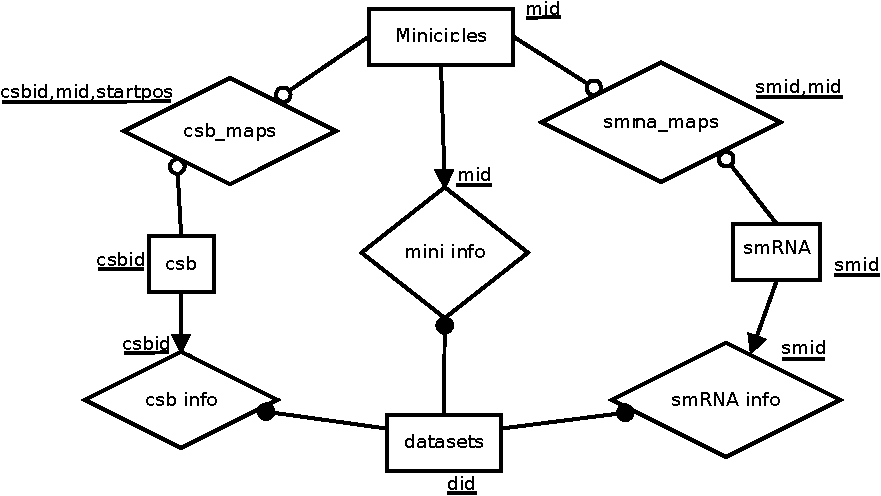
\includegraphics[width=.8\textwidth]{ERdiagram-crop.pdf}
    
\end{section}


\begin{section}{Tables}
    These are the tables we plan to implement in our project, with all fields listed. Primary keys are underlined,
    and foreign keys are italicized.

    \begin{itemize}
        \item \bfseries{CSB}: \underline{csbid}, sequence
        \item \bfseries{smallRNA}: \underline{smid}, sequence, copynumber
        \item \bfseries{dataset}: \underline{did}
        \item \bfseries{minicircles}: \underline{mid}, \textit{did}, sequence, clusternumber
        \item \bfseries{csb\_maps}: \underline{\textit{csbid},\textit{mid},startpos}, endpos, strandinfo, quality
        \item \bfseries{smrna\_maps}: \underline{\textit{smid}, \textit{mid}}, startpos, endpos, strandinfo, quality
    \end{itemize}
    
    As indicated by the ER diagram above we will have tables for smRNAs, minicircles, CSBs, datasets, and the maps of both 
    CSBs and smRNAs onto minicircles. These last two tables represent many-to-many relationships, and so they need their own 
    table. The relationships between our three sequence tables (minicircles, smRNAs, and CSBs) and the dataset table are all one to
    many, as each sequence may only belong to one dataset, a dataset being here defined as describing the origin of the sequences,
    the platform they were sequenced on, and other similar metadata. This relationship will be contained in the table structure 
    by having a dataset field holding a \underline{did} in each of these sequence tables. 

    For all of the sequence data tables (CSB, smallRNA, minicircles) the ID being used is a pre-supplied ID, which we are going
    to pull from the FASTA files containing our dataset on data import.

    \begin{subsection}{Indexes}
        We plan to use the following indexes on our tables:

        \begin{itemize}
            \item \bfseries{CSB}: primary key index on csbid
            \item \bfseries{smallRNA}: primary key index on smid
            \item \bfseries{dataset}: primary key index on did
            \item \bfseries{minicircles}: primary key index on mid
            \item \bfseries{csb\_maps}: Unique index on (csbid,mid,startpos)
            \item \bfseries{smrna\_maps}: Unique index on (smid,mid)
        \end{itemize}

        As we refine our queries and develop the web interface to our database it is likely that we will add to this and adopt
        other indexes.

    \end{subsection}



\end{section}

\begin{section}{Three SQL Queries}

    Here we present three sample SQL queries which could be used to answer a particular question about the data contained in our
    database.

    \begin{subsection}{Minicircle in largest cluster}
        Here we'd like to find the minicircle that belongs in the largest cluster, and return the minicircle id, the sequence,
        and the cluster number.

        \begin{lstlisting}
        SELECT mid, sequence, clusternum
        FROM minicircles
        GROUP BY clusternum
        ORDER BY count(*) DESC
        LIMIT 1;
        \end{lstlisting}
    \end{subsection}

    \begin{subsection}{All minicircles containing `csb3'}
        Now we'd like to find all of the minicircles which contain the CSB `csb3', and we'd like to return the minicircle id, the 
        minicircle sequence, and the cluster number:

        \begin{lstlisting}
        SELECT m.mid, m.sequence, m.clusternum
        FROM csb\_maps c NATURAL JOIN minicircle m
        WHERE c.csbid = 'csb3';
        \end{lstlisting}
    \end{subsection}

    \begin{subsection}{All smRNAs mapping to cluster 4 minicircles}
        We want to find all the smRNAs which map to minicircles that are in cluster 4, and return the minicircle id, the smRNAid, 
        and the smRNA sequence:

        \begin{lstlisting}
        SELECT m.mid, s.smid, s.sequence
        FROM smrna\_maps s NATURAL JOIN minicircles m
        WHERE m.clusternum = 4;
        \end{lstlisting}

    \end{subsection}
\end{section}

\begin{section}{External data processing}
    \begin{itemize}
        \item Clustalw2 will be used to perform multiple sequence alignment on a specified cluster number. Multiple sequence 
            alignments are computed on the fly when the user specifies an input cluster number.
        \item Alignment of smallRNA to minicircles was done using Bowtie2. This alignment is precomputed and stored in the 
            database.
        \item Cluster assignments to each minicircle was done using BLAST for each pairwise minicircle sequences, then clustered 
            as connected components. The clustering is precomputed and cluster assignments are stored in the database.
    \end{itemize}
\end{section}

\begin{section}{Links to Other databases}
    The data for our database comes from the following datasets:

    \begin{itemize}
        \item Minicircles published from Hong/Simpson Paper: http://dna.kdna.ucla.edu/tbrucei/Default.htm
        \item Curated list of T.brucei minicircles from Genbank. We have the fasta file containing all the sequences 
            from Genbank available to download.
        \item KISS database: reference link to another database that contains minicircles and guideRNA mappings: 
            http://gmod.mbl.edu/kiss/
    \end{itemize}

    We will link back to the Genbank sequences we use.

\end{section}

\begin{section}{Graphical Output}
    An overview of our plans for graphical output:

    \begin{itemize}
        \item Display multiple sequence alignments for minicircle reads belonging to a specified cluster (colorcoded by bases).
        \item Display alignment of smallRNA that maps to a specified minicircle. We will show the minicircle sequence as a 
            single track, then below the minicircle track, we will show the smallRNA sequences, aligned by the start and end 
            positions of where the smallRNA maps to the given minicircle. 
    \end{itemize}

\end{section}
            
\begin{section}{Data Download}
    We plan to offer the ability for users of our database to download data from it:

    \begin{itemize}
        \item After the user runnings a specific query to narrow down the list of minicircles of interest (ie. by CSB mapping or 
            clusternumber), there will be an option to download the minicircles from the query in fasta format. We will also 
            provide the option to download the smallRNA alignments that map to the minicircles of interest (alignment file in 
            BED format, smallRNA sequences in fasta format). 
        \item The user will be able to download the multiple sequence alignment file for a specified cluster (file in aln 
            format, output from clustalw2)
    \end{itemize}

\end{section}



    



        
            

















\end{document}
